
\documentclass[prb,reprint]{revtex4-2}

\usepackage{amsmath}    % need for subequations
\usepackage{graphicx}   % need for figures
\usepackage{verbatim}   % useful for program listings
\usepackage{color}      % use if color is used in text
\usepackage{subfigure}  % use for side-by-side figures
\usepackage{hyperref}   % use for hypertext links, including those to external
\raggedbottom           % don't add extra vertical space
\begin{comment}
\end{comment}

\bibliographystyle{apsrev4-2}

\begin{document}

\title{
    Machine-learned embedded atom method
}

\author{Xin Chen, 
        Li-Fang Wang, 
        De-Ye Lin$^\mathrm{*}$, 
        Hai-Feng Song$^\mathrm{*}$}

\affiliation{
    Institute of Applied Physics and Computational Math, 
    Beijing 100088, China}

\affiliation{
    CAEP Software Center for High Performance Numerical Simulation, 
    Beijing 100088, China}

% % % % % % % % % % % % % % % % % % % % % % % % % % % % % % % % % % % % % % % %
% 
% Abstract
%
% % % % % % % % % % % % % % % % % % % % % % % % % % % % % % % % % % % % % % % %
\begin{abstract}
\end{abstract}

\maketitle

% % % % % % % % % % % % % % % % % % % % % % % % % % % % % % % % % % % % % % % %
% 
% Section 1. Introduction
%
% % % % % % % % % % % % % % % % % % % % % % % % % % % % % % % % % % % % % % % %
\section{Introduction}
\label{sec:introduction}

Atomistic modeling plays a vital role in materials science. \textit{ab initio} 
calculation or force-field based molecular dynamics simulation (MD) are 
effective ways to study, understand or predict chemical and physical properties 
of materials. \textit{ab initio} approaches are generally much more precise but 
they are rarely used on large-scale metallic systems due to their extremely-high 
computation expenses. Physical model based empirical potential (force-field), 
such as the embedded-atom method (EAM), modified embedded-atom method (MEAM), 
bond-order potential (BoP), or angular-dependent potential (ADP), still plays 
the major role in long-time simulations and these empirical methods can achieve 
reasonable accuracy with much lower computation costs. Empirical potentials 
generally have very few learnable parameters and both microscopic observables 
(energy, forces, virial, etc.) and macroscopic observables (melting 
point, surface energy, etc.) can be used to tune these parameters. Finding 
optimal parameters of empirical potentials is always a challenging task. Global 
optimization (GO) approaches (Basin-Hopping, genetic algorithm, etc) are 
traditionally used to find the best possible parameters. However, the gradients 
of the losses with respect to model parameters are difficult or even impossible 
to calcualte. Hence, GO optimizations are generally not that effective.

In the last decade, machine learning (ML) has become one of the hottest 
topics in many research areas. In the materials science, researchers have made 
great efforts on developing ML models to describe atomic interactions. Such ML 
models are considered as machine learning interaction potentials (MLIPs). Until 
now, hundreds of MLIPs have been proposed. Among them, the symmetry-function 
based atomistic neural network (ANN) model, published by Parinello and Behler in 
2007, is still the most popular choice in modeling metallic interactions. 
The smooth overlap atomic positions descriptor based gaussian approximation 
potential (SOAP-GAP), developed by Bartòk et al, can give extremely accurate 
prediction results, although it's a bit computationally expensive. 
Recently, Thompson and co-workers proposed another quantum-accurate MLIP named 
the spectral neighbor analysis potential (SNAP) and it has been proven working  
on a broad range of metals and alloys. 

In many cases, MILPs can easily outperform state-of-art empirical potentials. 
Compared with empirical potentials, MLIPs generally have orders of magnitudes 
more model paramters. The redundant parameter space greatly reduces the 
difficulty of fitting complicated potential energy surfaces. But, to effectively 
train a MLIP and avoid overfitting, a large high-quality (versatile) training 
dataset is probably needed. However, MILPs \textbf{can really} take advantages 
of "big data" for two reasons. First, MLIPs typically only have 
\textit{basic} or \textit{simple} arithmetic operations. Thus, MILPs can be 
implemented within modern deep learning frameworks (TensorFlow, PyTorch, etc) 
so that the gradients of the total loss with respect to fitting parameters can 
be can obtained with the backpropagation algorithm automatically and 
efficiently. Second, MLIPs are mostly vectorizable. Hence, GPUs can be utilized
to significantly accelerate training and using of MILPs.

However, MLIPs also have challenges. The large parameter space and lack of 
physical background makes the "big data" a necessarity. The cost of dataset is 
non-negligible. Besides, even "big data" can only cover a small portion of real 
physical environments (temperature, external pressure, etc). Outside the 
training zone, the performances of MILPs may not that stable. For long-time 
molecular dynamics (MD) simulations of large-scale ($10^5$ or more) systems, 
computation efficiency also becomes a major concern. Recent benchmark tests 
suggest that MILPs are still too expensive. At present, most MLIPs are used to 
examine small to medium ($10^3$ to $10^4$) systems.

In this work, instead of designing new atomic descriptors, we chose a new route 
to develop MLIP: combining machine learning with empirical potentials. We 
successfully implemented EAM and its variant ADP within TensorFlow so that 
machine learning approaches can be used directly to tune EAM and ADP potentials. 
Our results suggest ML-EAM or ML-ADP can be as precise as the SNAP machine 
learning method. 

This paper is organized as follows. Section \ref{sec:method} describes the 
theoretical background of this work, including the formalism of the embedded 
atom method and algorithms and details of the machine learned EAM. 
Section \ref{sec:results} summarizes the training results and the optimal 
parameters. Applications of the new potentials are discussed in 
Section \ref{sec:discussions}.

% % % % % % % % % % % % % % % % % % % % % % % % % % % % % % % % % % % % % % % %
% 
% Section 2. Method
%
% % % % % % % % % % % % % % % % % % % % % % % % % % % % % % % % % % % % % % % %
\section{Method}
\label{sec:method}


% ------------------
% Section 2.A Theory
% ------------------
\subsection{Theory}
\label{sec:theory}

In the original EAM formalism, the total energy, $E^{total}$, is the sum of 
atomic energies:
\begin{align}
E^{total} = & \sum_{i}^{N}{E_{i}} \nonumber \\
\label{eq:eam_total_energy}
= & \sum_{i}^{N}{F_{a}(\rho_i)} + 
    \frac{1}{2}\sum_{i}^{N}{\sum_{j \neq i}^{r_{ij} < r_c}{
    \phi_{ab}(r_{ij})
}}
\end{align}
where $r_c$ is the cutoff radius, $a$ and $b$ represents species of atoms $i$ 
and $j$, $\phi_{ab}(r_{ij})$ is energy of the pairwise interaction between $i$ 
and $j$, $F_{a}(\rho_{i})$ is the embedding energy and $\rho_{i}$ is the local 
electron density of atom $i$. $\rho_{i}$ can be calculated with the following 
equation:
\begin{equation}
\label{eq:rho_eam}
\rho_{i} = \sum_{j}^{r_{ij} < r_{c}}{
    \rho_{b}(r_{ij})
}
\end{equation}
where $\rho_{b}$ is the electron density function of specie $b$. In the 
Finnis-Sinclair model, the electron density has a slightly modified form:
\begin{equation}
\label{eq:rho_fs}
\rho_{i}^{\mathrm{FS}} = \sum_{j}^{r_{ij} < r_{c}}{
    \rho_{ab}(r_{ij})
}
\end{equation}
$F$, $\rho$ and $\phi$ can be either parameterized functions or cubic splines.

The original EAM formalism does not inlcude angular-dependent interactions. To 
fix this problem, Baskes modified the original EAM and got MEAM (modified 
embedded-atom method), Lenosky proposed an alternative spline-based interpretion 
of MEAM  while Mishin developed the angular-dependent potential (ADP). The ADP 
formalism introduces three additional terms to the total energy:
\begin{align}
\label{eq:adp}
E^{total} 
& = E^{\mathrm{EAM}} \nonumber \\
& + \frac{1}{2}\sum_{i}{\sum_{\alpha}{(\mu_{i}^{\alpha})^2}} \nonumber \\
& + \frac{1}{2}\sum_{i}{
    \sum_{\alpha}{\sum_{\beta}{(\lambda_{i}^{\alpha\beta})^2}}} \nonumber \\
& - \frac{1}{6}\sum_{i}{\nu_{i}^{2}}
\end{align}
These terms represent non-central bonding contributions and they can be computed
with the following equations:
\begin{align}
\label{eq:adp_mu}
\mu_{i}^{\alpha} & = \sum_{j \neq i}{\mu_{ab}(r_{ij}) r_{ij}^{\alpha}} \\
\label{eq:adp_lambda}
\lambda_{i}^{\alpha\beta} & = \sum_{j \neq i}{
    \omega_{ab}(r_{ij}) r_{ij}^{\alpha}r_{ij}^{\beta}} \\
\label{eq:adp_nu}
\nu_{i} & = \sum_{\alpha}{\lambda_{i}^{\alpha\alpha}}
\end{align}
where $\mu_{ab}(r)$ and $\omega_{ab}(r)$ can be viewed as measures of the 
strengths of dipole and quadrupole interactions.

% -----------
% Section 2.B Transformation
% -----------
\subsection{Transformation}
\label{sec:transformation}

To integrate EAM/ADP with machine learning, the original total energy expression 
(Equation \ref{eq:eam_total_energy}) must be transformed to a vectorizable form. 
Without loss of generality, we take the binary alloy, AB, to demonstrate how to 
do the transformation.

\newcommand{\niaa}{N_{i}^{\mathrm{AA}}}
\newcommand{\niab}{N_{i}^{\mathrm{AB}}}
\newcommand{\njbb}{N_{j}^{\mathrm{BB}}}
\newcommand{\njba}{N_{j}^{\mathrm{BA}}}
\newcommand{\riaa}{\vec{\mathbf{r}}_{i}^{\mathrm{AA}}}
\newcommand{\riab}{\vec{\mathbf{r}}_{i}^{\mathrm{AB}}}
\newcommand{\ribb}{\vec{\mathbf{r}}_{i}^{\mathrm{BB}}}
\newcommand{\riba}{\vec{\mathbf{r}}_{i}^{\mathrm{BA}}}
\newcommand{\namax}{N_{\mathrm{A}}^{\mathrm{max}}}
\newcommand{\nbmax}{N_{\mathrm{B}}^{\mathrm{max}}}
\newcommand{\nnl}{N^{\mathrm{nl}}}
\newcommand{\nnli}{N^{\mathrm{nl}}_i}

Suppose the cutoff radius $r_c$ is fixed, the energy of atom $i$ of specie $A$ 
can be calculated with the following expanded equation:
\begin{align}
\label{eq:e_atom_phase_1}
E_{i}^{A} 
= & 
\frac{1}{2}\sum_{j\neq i}^{\niaa}\phi_{\mathrm{AA}}(r_{ij}) +
\frac{1}{2}\sum_{j\neq i}^{\niab}\phi_{\mathrm{AB}}(r_{ij}) \nonumber \\
+ & F_{\mathrm{A}}\left(
    \sum_{j\neq i}^{\niaa}{\rho_{\mathrm{A}}(r_{ij})} +
    \sum_{j\neq i}^{\niab}{\rho_{\mathrm{B}}(r_{ij})} 
\right)
\end{align}
where $\niaa$ represents the number of A-type neighors of atom $i$ and 
$\niab$ represents the number of B-type neighors. For atom $j$ of specie $B$, we
can also write a similar form. 
\begin{align}
\label{eq:e_atom_phase_1}
E_{j}^{B} 
= & 
\frac{1}{2}\sum_{i \neq j}^{\njbb}\phi_{\mathrm{BB}}(r_{ij}) +
\frac{1}{2}\sum_{i \neq j}^{\njba}\phi_{\mathrm{AB}}(r_{ij}) \nonumber \\
+ & F_{\mathrm{B}}\left(
    \sum_{j\neq i}^{\njbb}{\rho_{\mathrm{B}}(r_{ij})} +
    \sum_{j\neq i}^{\njba}{\rho_{\mathrm{A}}(r_{ij})} 
\right)
\end{align}
When $r_c$ is fixed, $\niaa$, $\niab$, $\njbb$ and $\njba$ are all constants and
$\nnli$ is the maximum of these numbers. Finally, we can pre-determine the 
maximum neighor list size $\nnl$:
\begin{equation}
\label{eq:nnl}
\nnl = \max{\left(\nnli\right)}
\end{equation}
$\nnl$ is also a constant in the training phase because both the training 
dataset and $r_c$ are fixed.

Next, assume $H(x)$ represents the heaviside step function:
\begin{equation}
\label{eq:heaviside}
H(x) = \begin{cases}
    1 & x > 0 \\
    0 & x \leq 0 \\
\end{cases}
\end{equation}
then the pairwise term can be transformed to:
\begin{align}
\sum_{j\neq i}^{\niaa}\phi_{\mathrm{AA}}(r_{ij}) = &
\sum_{j\neq i}^{\niaa}\phi_{\mathrm{AA}}(r_{ij}) \cdot 1 + 
\sum_{j\neq i}^{\nnl - \niaa}\phi_{\mathrm{AA}}(0) \cdot 0 \nonumber \\
= & \phi_{\mathrm{AA}}(\vec{\mathbf{r}}_{i}^{\mathrm{AA}})^T
H(\vec{\mathbf{r}}_{i}^{\mathrm{AA}})
\end{align}
where $\vec{\mathbf{r}}_{i}^{\mathrm{AA}}$ is a $\nnl$-length column vector 
whose last $\nnl - \niaa$ elements are zeros.

We can write Equation \ref{eq:e_atom_phase_1} in an equivalent expression:
\begin{align}
E_{i}^{\mathrm{A}} 
\label{eq:e_atom_A}
= &
\frac{1}{2}\left( 
    \phi_{\mathrm{AA}}(\vec{\mathbf{r}}_{i}^{\mathrm{AA}})^T
    H(\vec{\mathbf{r}}_{i}^{\mathrm{AA}}) +
    \phi_{\mathrm{AB}}(\vec{\mathbf{r}}_{i}^{\mathrm{AB}})^T
    H(\vec{\mathbf{r}}_{i}^{\mathrm{AB}})
\right) \nonumber \\
+ &
F_{\mathrm{A}}\left( 
    \rho_{\mathrm{AA}}(\vec{\mathbf{r}}_{i}^{\mathrm{AA}})^T
    H(\vec{\mathbf{r}}_{i}^{\mathrm{AA}}) +
    \rho_{\mathrm{AB}}(\vec{\mathbf{r}}_{i}^{\mathrm{AB}})^T
    H(\vec{\mathbf{r}}_{i}^{\mathrm{AB}})
\right)
\end{align}
Here $\vec{\mathbf{r}}_{i}^{\mathrm{AB}}$ is also a $\nnl$-length vector. For 
atom $j$ of specie $B$, we can also derive its energy $E^{\mathrm{B}}_{j}$:
\begin{align}
E_{j}^{\mathrm{B}}
\label{eq:e_atom_B}
= &
\frac{1}{2}\left( 
    \phi_{\mathrm{BB}}(\vec{\mathbf{r}}_{j}^{\mathrm{BB}})^T
    H(\vec{\mathbf{r}}_{j}^{\mathrm{BB}}) +
    \phi_{\mathrm{BA}}(\vec{\mathbf{r}}_{j}^{\mathrm{BA}})^T
    H(\vec{\mathbf{r}}_{j}^{\mathrm{BA}})
\right) \nonumber \\
+ &
F_{\mathrm{A}}\left( 
    \rho_{\mathrm{BB}}(\vec{\mathbf{r}}_{j}^{\mathrm{BB}})^T
    H(\vec{\mathbf{r}}_{j}^{\mathrm{BB}}) +
    \rho_{\mathrm{BA}}(\vec{\mathbf{r}}_{j}^{\mathrm{BA}})^T
    H(\vec{\mathbf{r}}_{j}^{\mathrm{BA}})
\right)
\end{align}

Since $\riaa$, $\riab$, $\ribb$ and $\riba$ all have the same length ($\nnl$), 
we can use a (redundant) matrix, $\mathbf{g}_{i}$, to describe all neighbors of 
atom $i$:
\begin{equation}
\mathbf{g}_i = \begin{bmatrix}
    \riaa & \riab & \ribb & \riba \\
\end{bmatrix}
\end{equation}
$\mathbf{g}_i$ is a $\nnl \times 4$ matrix. If the specie of atom $i$ is A, only
the first two columns have non-zero values. Similarly, the last two columns will
have non-zeros values if atom $i$ is a B-type atom. In fact, $\mathbf{g}_i$ can
be viewed as the EAM descriptors for atom $i$. Hence, each structure can be 
expressed with a 3D matrix, $\mathbf{G}$ , of shape $N \times \nnl \times 4$.

During the training phase, the maximum appearances of element A and B in any 
structure ($\namax$ and $\nbmax$) are also constants. Thus, any $\mathbf{G}$ can 
be expanded to a $(\namax + \nbmax) \times \nnl \times 4$ matrix $\mathbf{G}'$ 
by zero-padding. In summary, arbitrary structure in the training dataset can be 
converted to a fixed-shape descriptor matrix $\mathbf{G}'$. 

For the ADP formalism, the corresponding transformation is almost the same 
except that $\mathbf{g}_{i}^{\mathrm{adp}}$ should also include the XYZ 
components of $\vec{\mathbf{r}}_i$.

% -----------
% Section 2.C Functions
% -----------
\subsection{Functions}
\label{sec:functions}

In this work, we use the EAM potential published by Zhou, Johnson and Wadley 
(Zjw04) as an example to validate our machine learning approach. Zjw04 is a 
quite popular EAM potential. In the Zjw04 potential, the electron density 
function has the following form:
\begin{equation}
\label{eq:zjw04_rho}
\rho_{b}(r) = \frac{
    f_{e} \exp\left[ -\beta\left( r/r_{e} - 1 \right) \right]
}{
    1 + \left(r/r_{e} - \lambda\right)^{20}
}
\end{equation}
where $r_e$ is a constant equal to equilibrium spacing between nearest neighors, 
$f_{e}$, $\beta$, $\lambda$ are adjustable parameters. The pairwise potential 
between the same species can be computed with:
\begin{equation}
\label{eq:zjw04_phi_aa}
\phi_{aa}(r) = 
\frac{A \exp\left[ -\alpha\left( r/r_{e} - 1 \right) \right]}
     {1 + \left(r / r_{e} - \kappa\right)^{20}} - 
\frac{B \exp\left[ -\beta\left( r/r_{e} - 1 \right) \right]}
     {1 + \left(r / r_{e} - \lambda\right)^{20}}
\end{equation}
where $A$, $B$, $\alpha$ and $\kappa$ are also trainable parameters, $\beta$ and 
$\kappa$ are used in Equation \ref{eq:zjw04_rho} already. For the pairwise 
interaction between two atoms of different species, Zhou et al proposed an 
interpolation form:
\begin{equation}
\label{eq:zjw04_phi_ab}
\phi_{ab}(r) = \frac{1}{2}\left(
    \frac{\rho_{b}(r)}{\rho_{a}(r)}\phi_{aa}(r) +
    \frac{\rho_{a}(r)}{\rho_{b}(r)}\phi_{bb}(r) 
\right)
\end{equation}
The embedding function has a more complicated form as it requires to fit a much 
wider range of electron density values:
\begin{equation}
\label{eq:zjw04_embed}
F(\rho) = \begin{cases}
    \sum_{i=0}^{3}{F_{ni}\left( \frac{\rho}{\rho_n} - 1 \right)^{i}} &
    \rho < \rho_{n} \\
    \sum_{i=0}^{3}{F_{i}\left( \frac{\rho}{\rho_e} - 1 \right)^{i}} &
    \rho_{n} \leq \rho < \rho_{0} \\
    F_{e}\left[ 
        1 - \eta\ln\left( \frac{\rho}{\rho_s}\right) 
    \right](\frac{\rho}{\rho_s})^{\eta} & \rho_{0} \leq \rho
\end{cases}
\end{equation}
where $F_{ni}$, $F_{i}$, $\rho_e$, $\rho_s$, $\eta$ and $F_{e}$ are trainable 
parameters, $\rho_n=0.85\rho_e$ and $\rho_0=1.15\rho_e$. For each metal, there 
are 15 adjustable parameters. The original embedding potential is a stepwise 
function. Thus, the minimization requires some tricks to ensure its continuity.
To make it simpler, we slightly modified Equation \ref{eq:zjw04_embed}:
\begin{align}
\label{eq:zjw04xc_embed}
F(\rho) 
= & c_1 \cdot
\sum_{i=0}^{3}{F_{ni}\left( \frac{\rho}{\rho_n} - 1 \right)^{i}} \nonumber \\
+ & c_2 \cdot 
\sum_{i=0}^{3}{F_{i}\left( \frac{\rho}{\rho_e} - 1 \right)^{i}} \nonumber \\
+ & c_3 \cdot
F_{e}\left[1 - \eta\ln\left( \frac{\rho}{\rho_s}\right)\right]
(\frac{\rho}{\rho_s})^{\eta} \\
\label{eq:frho_c1}
c_{1} = & \frac{1}{1 + e^{-2\left(\rho_{n} - \rho\right)}} \\
\label{eq:frho_c3}
c_{3} = & \frac{1}{1 + e^{-2\left(\rho - \rho_{0}\right)}} \\
c_{2} = & 1 - c_1 - c_3
\end{align}
$\omega_1$ and $\omega_3$ are just damping factors calculated by the sigmoid 
functions (Equations \ref{eq:frho_c1} and \ref{eq:frho_c3}).

The dipole ($\mu_{ab}$) and quadrupole ($\lambda_{ab}$) functions have the same 
form (developed by Mishin):
\begin{align}
\label{eq:adp_dipole}
\mu_{ab}(r) & = \left[
    d_{1}^{ab} \exp\left( -d_{2}^{ab}r \right) + d_{3}^{ab}
\right] \psi\left( \frac{r - r_{0}}{r_{h}} \right) \\
\omega_{ab}(r) & = \left[
    q_{1}^{ab} \exp\left( -q_{2}^{ab}r \right) + q_{3}^{ab}
\right] \psi\left( \frac{r - r_{0}}{r_{h}} \right)
\end{align}
where $d_{i}$, $q_{i}$, $r_0$ and $r_{h}$ are trainable parameters and $\psi(x)$
is a damping function:
\begin{equation}
\label{eq:mishin_cutoff}
\psi(x) = \begin{cases}
    0 & x \ge 0 \\
    \frac{x^4}{1 + x^4} & x < 0 
\end{cases}
\end{equation}

% -----------
% Section 2.D Physical constraints
% -----------
\subsection{Physical constraints}
\label{sec:constraints}

Physical constraints are quite common in fitting traditional empirical 
potentials. Physical constraints are typically static (cohesive energy, elastic 
constants, etc) collected from experiments and they can be very effective when 
training data is limited. For example, the cohesive energy, bulk modulus, 
vacancy formation energy and other constraints were used to develop the original 
Zjw04 potential. Mishin et al adopted the Rose universal equation of state to 
ensure the performaces of his ADP potentials in the high pressure region. 
However, such constraints are really rare in developing MILPs. One possible 
explanation may be these constraints are generally derived properties and 
implementing them in the loss function are technically difficult.

In this work, we successfully integrated two constraints into the total loss:
the Rose equation of state (EOS) constraint and the elastic tensor constraint. 
These two losses will be discussed later. The details of their implementations 
will be described in another paper.

The Rose constraint incoporates the universal equation of state (Rose et al) 
into the total loss function. The Mishin-modified equation 
\begin{equation}
\label{eq:rose_eos}
E(x) = E_{0}\left[
    1 + \alpha x + \beta \alpha^3 x^3 \frac{2x + 3}{(x - 1)^2} \right]
    e^{-\alpha x}
\end{equation}
is used because the original form tends to underestimate energies under high 
pressures. In Equation \ref{eq:rose_eos}, $E_{0}$ is the energy of the 
equilibrium structure, $x = a / a_{0} - 1$ is the relative isotropic scaling 
factor ($a$ is the lattice constant), $\beta$ is a chosen parameter and 
\begin{equation}
\label{eq:rose_alpha}
\alpha = \sqrt{-\frac{9 V_{0} B }{E_{0}}}
\end{equation}
where $V_0$ is the equilibrium volume and $B$ is the bulk modulus. The adoption
of the Rose constraint guarantees the exact predictions of bulk modulus and 
the energy-volume curve. The loss of the Rose EOS constraint 
$\mathbf{L}^{\mathrm{Rose}}$  is measured as the 2-norm of the energy 
differences between $E(x)^{\mathrm{dft}}$ and their corresponding predicted 
$E(x)$: 
\begin{equation}
\label{eq:rose_loss}
\mathbf{L}^{\mathrm{Rose}} = \sum_{\Omega}{
    \sqrt{\sum_{i}{\left(E(x_i) - E(x_i)^{\mathrm{dft}}\right)^2}}
}
\end{equation}
Here $\Omega$ denotes all selected crystals. In this work, for each included 
crystal, we use the same choices of $x$: 
$x_{i} = x_{0} + \Delta x \cdot i, x_{0} = -0.1, N_{t}^{\mathrm{max}} = 20, 
\Delta x=0.01$. In this work, $\beta^{\mathrm{Ni}}$ is 0.005 and 
$\beta^{\mathrm{Mo}}$ is 0.150.
 
Elastic tensor is also a popular constraint for tuning empirical potentials but 
rarely used directly in optimizing MILPs. Shyue Ping Ong used this constraint in 
the outer loop (the global optimization based property-matching step) to find 
optimal parameters of SNAP potentials. 

In this work, we successfully find a way to use elastic tensor directly as a 
constraint. Given an equilibrium crystal structure, its elastic constant 
$c_{ijkl}$ can be derived from $E^{total}$ directly:
\begin{align}
\label{eq:virial}
V \cdot \epsilon & = -\mathbf{F}^{T}\mathbf{R} + \left(
    \frac{\partial E^{total}}{\partial \mathbf{h}}\right)^T \mathbf{h} \\ 
\label{eq:cijkl}
c_{ijkl} |_{\epsilon \to 0, \mathbf{F} \to 0} & = \frac{1}{V}\left[
    \left( 
        \frac{\partial{\epsilon_{ij}}}{\partial{\mathbf{h}}}
    \right)^{\mathrm{T}}\mathbf{h}
\right]_{kl}
\end{align}
where $V$ is the volume, $\epsilon$ is the $3 \times 3$ virial stress tensor, 
$\mathbf{h}$ is the \textit{row-major} $3 \times 3$ lattice tensor, $\mathbf{F}$ 
and $\mathbf{R}$ are $N \times 3$ matrices representing the total forces and 
atomic positions.

In this work, the loss $\mathbf{L}^{\mathrm{elastic}}$ contributed by the 
elastic tensor is also measured by the RMSE between $c_{ijkl}$ and 
$c_{ijkl}^{\mathrm{dft}}$:
\begin{align}
\label{eq:cijkl_loss}
\mathbf{L}^{\mathrm{elastic}} 
& = \sum_{\Omega}{\left(
    \omega_{\Omega} \cdot \mathbf{RMSE}_{\Omega} 
    + ||\epsilon|| + ||\mathbf{F}||
\right)}
 \\
\label{eq:cijkl_loss_gate}
\omega_{\Omega} & = \mathbf{ReLU}(\mathbf{MAE}_{\Omega} - \tau) \\
\label{eq:relu}
\mathbf{ReLU}(x) & = \begin{cases}
    x & x \ge 0 \\
    0 & x < 0
\end{cases}
\end{align}
where $\sum_{\Omega}$ loops through all included crystals, 
$\mathbf{MAE}_{\Omega}$ and $\mathbf{RMSE}_{\Omega}$ are the mean absolute error 
and root mean squared error between predicted elastic constants and DFT elastic 
constants. $\tau$ is a pre-selected gate parameter. 
When $\mathbf{MAE}$ is below $\tau$, $\mathbf{L}^{\mathrm{elastic}}$ will not 
contribute to the total loss. In this work, $\tau$ is set to 2 GPa.

% -----------
% Section 2.E Implementation
% -----------
\subsection{Implementation}
\label{sec:implementation}

The implementation of the machine learned embedded atom mathod and the physical
constraints are beyond the scope of this work. The details will be discussed
in another paper. Here, we will give a brief description.

Both ML-EAM and ML-ADP are implemented within Google's TensorFlow. The 
virtual-atom approach (VAP) is adopted so that we can construct a computation 
graph from atomic positions to total energy directly. Thus, atomic forces 
(Equation \ref{eq:forces}) and virial stress (Equation \ref{eq:virial}) can be 
derived by the AutoGrad module of TensorFlow and calcualted automatically and 
efficiently. 
\begin{equation}
\label{eq:forces}
\mathbf{F} = -\frac{\partial E^{total}}{\partial \mathbf{R}}
\end{equation}
This direct computation graph also plays a key role in computing analytical 
elastic tensor (Equation \ref{eq:cijkl}) and the Rose loss 
(Equation \ref{eq:rose_eos}).
 
To find optimal parameters of the funcitons in section \ref{sec:functions}, the 
overall loss function shall be defined. Just like other machine learning tasks, 
the mini-batch stochastic gradient descent algorithm is used to minimize the 
loss function. Equation \ref{eq:loss} demonstrates the loss function used in 
this work:
\begin{align}
\label{eq:loss}
\mathbf{Loss} & = \sqrt{\frac{1}{N_{b}}\sum_{i=1}^{N_{b}}{\left(
    E_{i} - E_{i}^{\mathrm{dft}}
\right)^2}} \nonumber \\
& + \chi_{\mathrm{f}}\sqrt{
    \frac{1}{3\sum_{i}^{N_{b}}{N_i}}\sum_{i}^{N_b}{\sum_{j}^{N_i}{
        \sum_{\alpha}{
            \left(f_{ij\alpha} - f_{ij\alpha}^{\mathrm{dft}}\right)^2
        }
    }}
} \nonumber \\
& + \chi_{\mathrm{s}}\sqrt{\frac{1}{6N_b}\sum_{i}^{N_b}{
    \sum_{j}^{6}{
        \left(
            \epsilon^{\mathrm{voigt}}_{j} - \epsilon^{\mathrm{voigt,dft}}_{j}
        \right)^2
    }
}} \nonumber \\
& + \chi_{\mathrm{rose}}\mathbf{L}^{\mathrm{Rose}} 
+ \chi_{\mathrm{elastic}}\mathbf{L}^{\mathrm{elastic}}
\end{align} 
where $N_{b}$ is the batch size and $N_i$ is the number of atoms in structure 
$i$. $\chi_{\mathrm{f}}$, $\chi_{\mathrm{s}}$, $\chi_{\mathrm{rose}}$ and 
$\chi_{\mathrm{elastic}}$ are overall weights of force, virial stress, rose EOS 
and elastic contributions. The superscript 'voigt' means that virial 
stress tensors should be converted to Voigt form. The Adam optimizer is used to 
minimize Equation \ref{eq:loss}. In most cases, we use 0.01 as the initial 
learning rate and the batch size ranges from 20 to 50. Since there are very few
adjustable parameters, the optimization typically needs very few epochs to 
converge. When the optimization is finished, the corresponding Lammps setfl 
potential file will be exported.

% % % % % % % % % % % % % % % % % % % % % % % % % % % % % % % % % % % % % % % %
% 
% Section 3. Results
%
% % % % % % % % % % % % % % % % % % % % % % % % % % % % % % % % % % % % % % % %
\section{Results}
\label{sec:results}

The publicly Ni-Mo dataset is used to evaluate our approach. This dataset is 
provided by Shyue Ping Ong. It contains 3973 different Ni-Mo solids. All 
calculations were done by VASP with the PBE functional and the projector 
augmented-wave approach. 

The melting points $T_{m}$ of bcc Mo and fcc Ni were measured with the 
solid-liquid coexistence approach. For fcc Ni, $30 \times 10 \times 10$ 
supercells were used and for bcc the supercells were $30 \times 15 \times 15$. 
The time step was set to 1 fs. The simulation for each temperature was carried 
out for 300 ps.

% % % % % % % % % % % % % % % % % % % % % % % % % % % % % % % % % % % % % % % %
% 
% Section 3.A
%
% % % % % % % % % % % % % % % % % % % % % % % % % % % % % % % % % % % % % % % %
\subsection{Ni}
\label{sec:elementary_Ni}

% % % % % % % % % % % % % % % % % % % % % % % % % % % % % % % % % % % % % % % %
% 
% Figure: Ni - EOS
%
% % % % % % % % % % % % % % % % % % % % % % % % % % % % % % % % % % % % % % % %
\begin{figure}[htp]
\centering
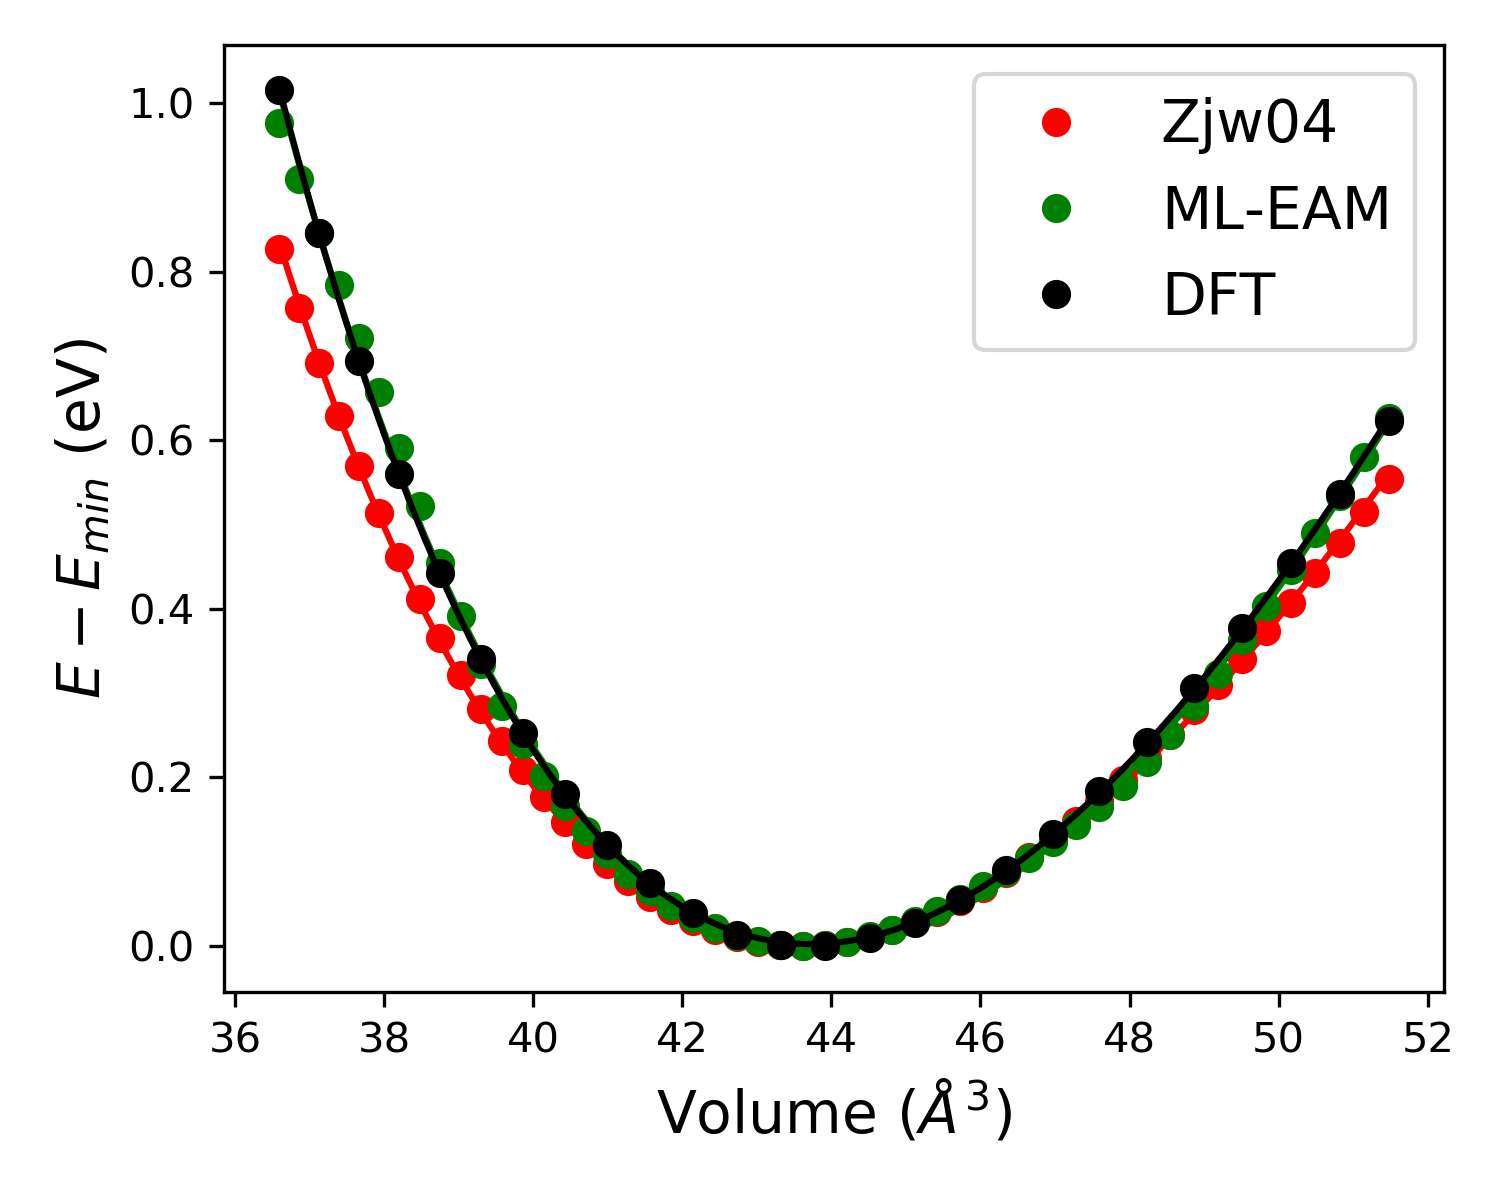
\includegraphics[scale=0.65]{figures/Ni_all_eos.png}
\caption{\label{fig:Ni_eam_eos} The energy-volume curves of the original EAM, 
SNAP, ML-EAM and DFT for the fcc Ni.}
\end{figure}

We first use the elementary fcc Ni dataset to show our approach. This dataset 
has 461 structures in total. 400 were randomly selected to form the training 
subset. In this experiment, $\chi_{\mathrm{f}}$, $\chi_{\mathrm{rose}}$ and 
$\chi_{\mathrm{elastic}}$ were set to 1, 3 and 0.05 respectively. The batch size
was 25. Only the fcc Ni was included in $\Omega$ (Equation \ref{eq:rose_loss} 
and \ref{eq:cijkl_loss}).

Table \ref{table:elementary_Ni_mae} shows the MAEs of those models. The original 
EAM model already has an accepetable performace on this fcc dataset. Its energy 
MAE is 10.6 meV/atom and the force MAE is 0.06 eV/\AA. The MEAM performs 
slightly worse on this dataset with an energy MAE of 17.6 meV/atom and force MAE
of 0.08 eV/\AA. Our machine learning approach can further reduce the energy MAE 
to 4.1 meV/atom and the force MAE to 0.05 eV/\AA, which are much closer to the 
elementary SNAP Ni model.

Figure \ref{fig:Ni_eam_eos} plots the equation of state curves obtained with the 
DFT, SNAP, EAM and ML-EAM models. The whole fitting region ranges from 84\% to 
118\% of the equilibrium volume. The original EAM significantly underestimates 
the energy at both tensile and compress strains. However, our machine learning 
approach together with the Rose constraint can fix this problem. The 
energy-volume curve of ML-EAM overalps with the DFT curve very well for the 
entire fitting region. 

Table \ref{table:elementary_Ni} summerizes the predicted material properties of 
fcc Ni, including the melting point, the elastic constants, the vacancy 
formation energy $E_{v}$, the migration energy $E_{m}$ and the activation energy 
$E_{a}$. The original EAM already performs well on these properties. ML-EAM 
further improves the elastic constants. The errors were significantly reduced 
to around 1-2\%.

% % % % % % % % % % % % % % % % % % % % % % % % % % % % % % % % % % % % % % % %
% 
% Table: Ni - MAE
%
% % % % % % % % % % % % % % % % % % % % % % % % % % % % % % % % % % % % % % % %
\begin{table}[h]
\centering
\begin{tabular}{lcccc}
\hline
 MAE & SNAP & EAM & MEAM & ML-EAM \\
\hline
Energy (meV/atom) & 1.2 & 10.6 & 17.8 & 4.1 \\
Force (eV/\AA) & 0.05 & 0.06 & 0.08 & 0.05 \\
\hline
\end{tabular}
\caption{\label{table:elementary_Ni_mae} Comparion of the energy and force 
accuracy of the elementary SNAP Ni model, the original EAM, the MEAM and our 
ML-EAM.
}
\end{table}    

% % % % % % % % % % % % % % % % % % % % % % % % % % % % % % % % % % % % % % % %
% 
% Table: Ni - Material Properties
%
% % % % % % % % % % % % % % % % % % % % % % % % % % % % % % % % % % % % % % % %
\begin{table*}[htp]
\centering
\begin{tabular}{lcccccc}
\hline
    & DFT & SNAP & EAM & MEAM & ML-EAM & Exp. \\
\hline
$T_{m}$(K) & & 1785 & 1520 & 1765 & 1520 & 1728 \\
$c_{11}$ (GPa) & 276 & 276 (0.0\%) & 248 (-10.1\%) & 260 (-5.8\%) & 274 (-0.7\%) & 261 \\
$c_{12}$ (GPa) & 159 & 159 (0.0\%) & 147 (-7.5\%) & 151 (0.0\%) & 163 (2.5\%) & 151 \\
$c_{44}$ (GPa) & 132 & 132 (0.0\%) & 125 (-5.3\%) & 131 (0.0\%) & 131 (-0.8\%) & 132 \\
$E_{v}$ (eV) & 1.46 & 1.68 (15.1\%) & 1.68 (15.1\%) & 1.16 (-20.5\%) & 1.71 (17.1\%) & 1.54–1.80 \\
$E_{m}$ (eV) & 1.12 & 1.07 (-4.5\%) & 0.90 (-19.6\%) & 1.46 (30.5\%) & 0.87 (-22.3\%) & 1.01–1.48 \\
$E_{a} = E_{v} + E_{m} $ (eV) & 2.58 & 2.75 (6.6\%) & 2.58 (0.0\%) & 2.62 (1.6\%) & 2.58 (0.0\%) & 2.77–2.95 \\
\hline
\end{tabular}
\caption{\label{table:elementary_Ni} Comparison of the calculated and 
experimental material properties of elementary fcc Ni. $T_{m}$ is the melting 
point. $c_{ij}$ represents elastic constants. $E_{v}$ and $E_{m}$ are vacancy 
formation energy and migration energy, respectively. SNAP refers to the 
elementary Ni SNAP model.
}
\end{table*}

Figure \ref{fig:Ni_eam} compares the $rho(r)$, $F(\rho)$ and $\phi(r)$ functions
of ML-EAM with original Zjw04 EAM. The pairwise potential $\phi(r)$ almost 
remains the same while the embedding function $F(\rho)$ and the electron density 
function $\rho(r)$ changes significantly. Both $\rho(r)$ and $\phi(r)$ converge
to zero at around $r=4.8$ \AA, which is rougly 2 times of the equilibrium 
spacing between nearest neighbors.

% % % % % % % % % % % % % % % % % % % % % % % % % % % % % % % % % % % % % % % %
% 
% Figure: Ni - EAM - Plot
%
% % % % % % % % % % % % % % % % % % % % % % % % % % % % % % % % % % % % % % % %
\begin{figure*}[htp]
\centering
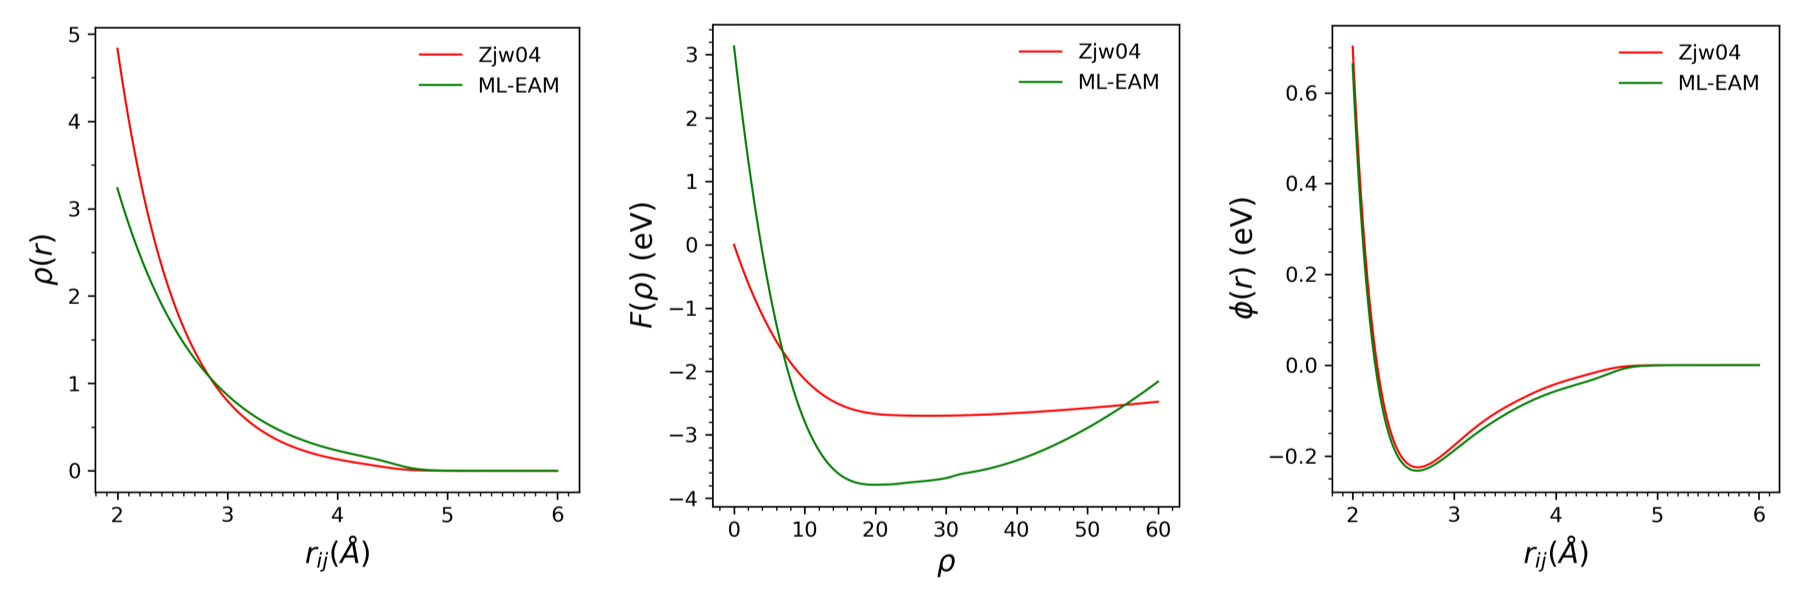
\includegraphics[scale=0.57]{figures/Ni_eam.png}
\caption{\label{fig:Ni_eam} $\rho(r)$, $F(\rho)$ and $\phi(r)$ of the original 
Zjw04 EAM and the machine learned EAM (ML-EAM).}
\end{figure*}


% % % % % % % % % % % % % % % % % % % % % % % % % % % % % % % % % % % % % % % %
% 
% Section 3.B
%
% % % % % % % % % % % % % % % % % % % % % % % % % % % % % % % % % % % % % % % %
\subsection{Mo}
\label{sec:elementary_Mo}

The second test example is bcc Mo. This dataset has 284 structures. 34 of 
them were used as the testing subset and the rest were used for training. 
The training settings were the same with fcc Ni. An ADP potential was also 
optimized for bcc Mo.

Table \ref{table:elementary_Mo_mae} summerizes the energy and force MAEs on the 
test subset. The original Zjw04 EAM performs significantly worse. The energy 

% % % % % % % % % % % % % % % % % % % % % % % % % % % % % % % % % % % % % % % %
% 
% Figure: Mo - EAM/ADP - Plot
%
% % % % % % % % % % % % % % % % % % % % % % % % % % % % % % % % % % % % % % % %
\begin{figure*}[htp]
\centering
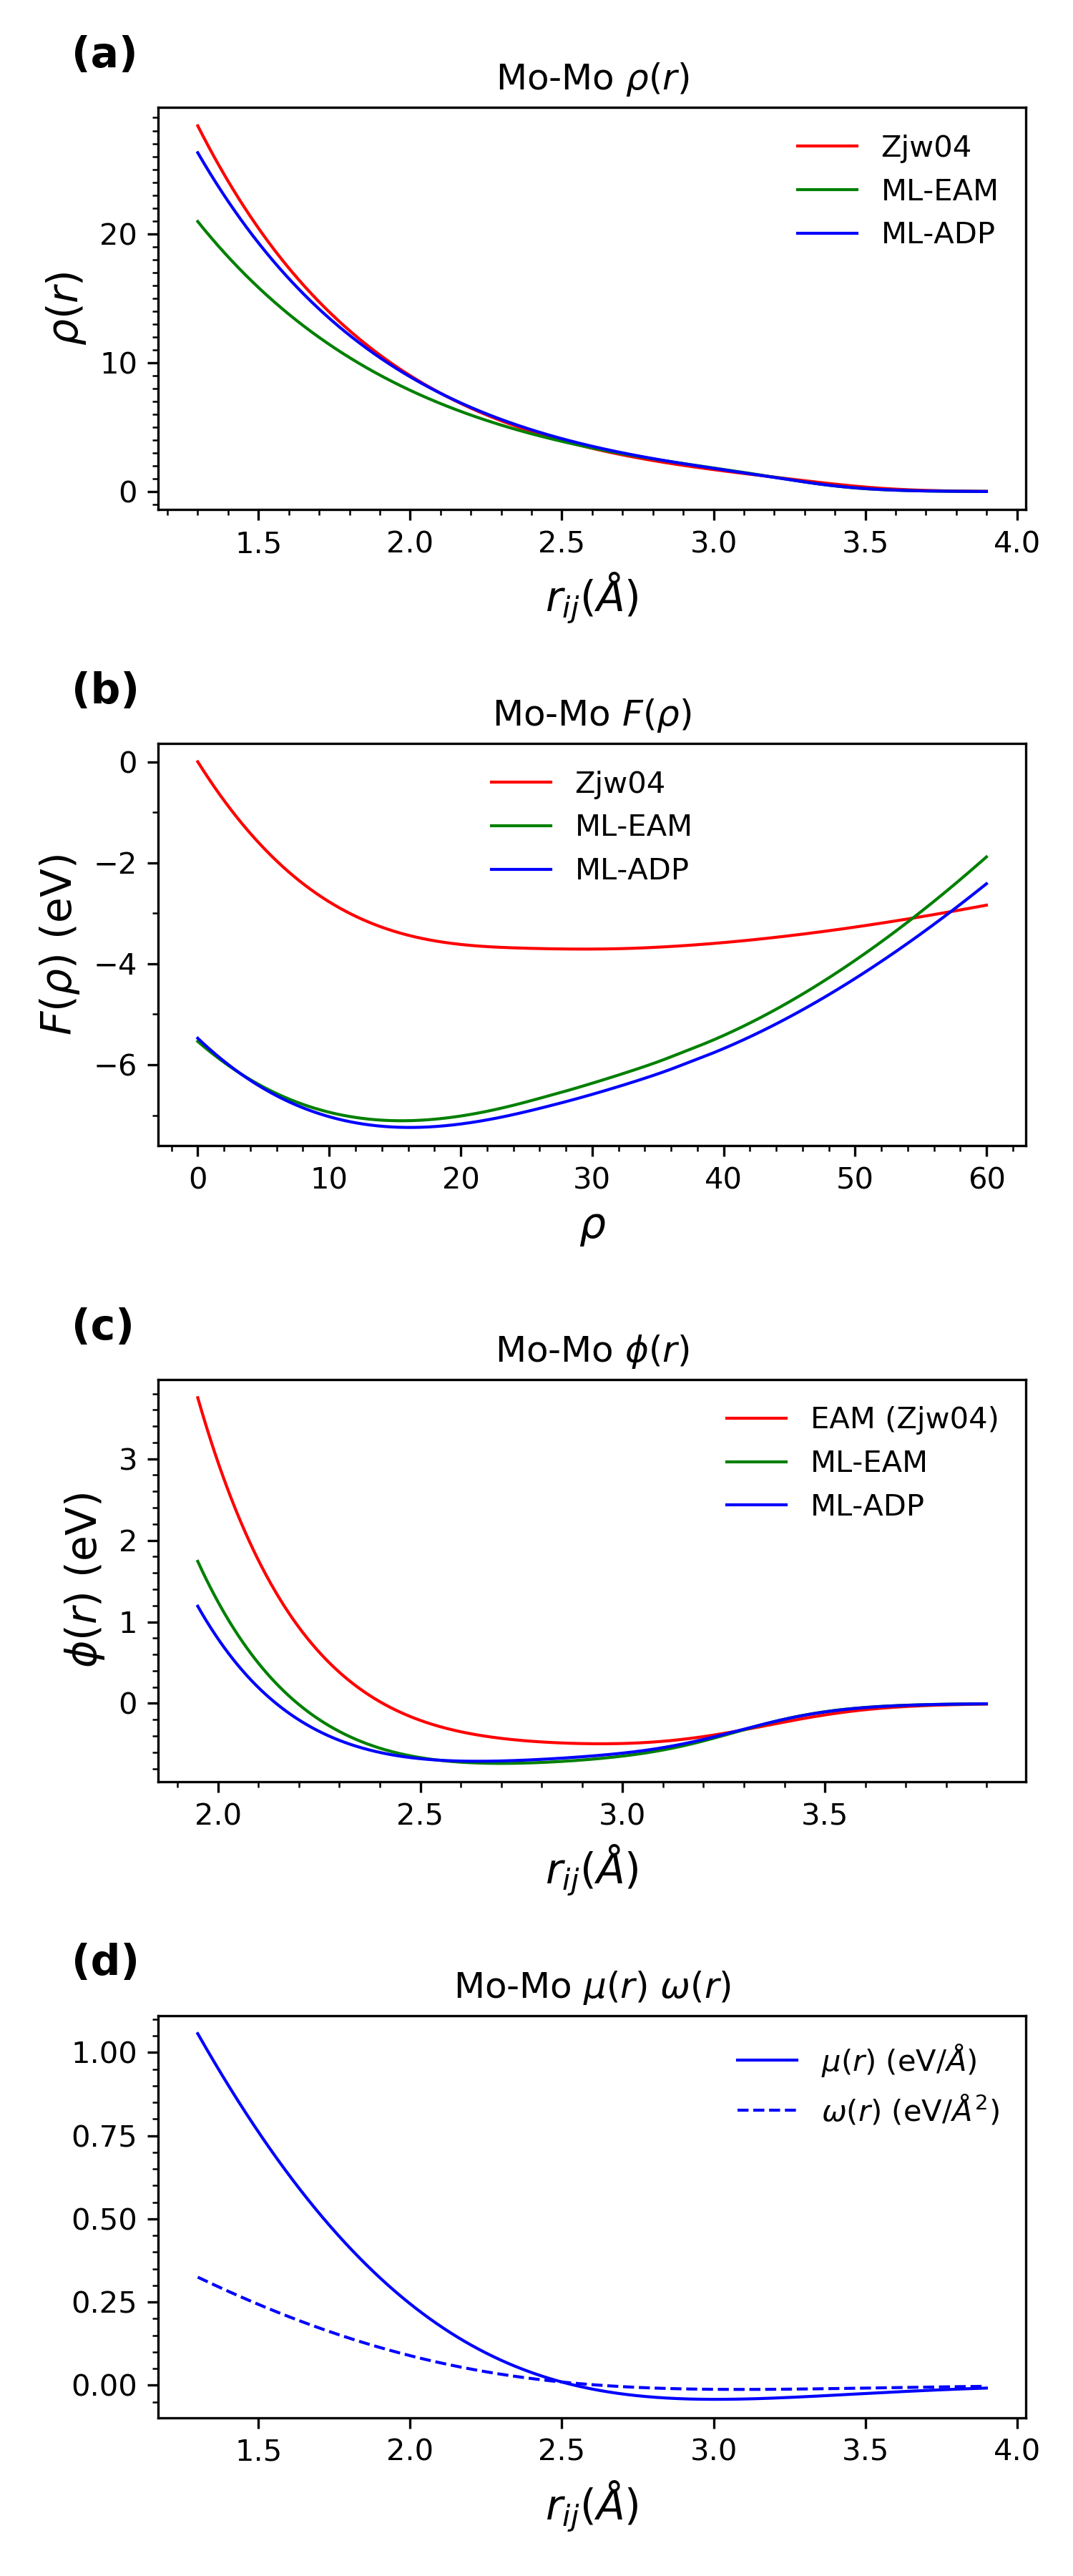
\includegraphics[scale=0.6]{figures/Mo_eam_adp.png}
\caption{\label{fig:Mo_eam_adp} $\rho(r)$, $F(\rho)$, $\phi(r)$ of the original 
Zjw04 EAM, ML-EAM and ML-ADP. \textbf{(d)} shows the $\mu(r)$ and $\omega(r)$ of 
ML-ADP.}
\end{figure*}

% % % % % % % % % % % % % % % % % % % % % % % % % % % % % % % % % % % % % % % %
% 
% Table: Mo - MAE
%
% % % % % % % % % % % % % % % % % % % % % % % % % % % % % % % % % % % % % % % %
\begin{table}[h]
\centering
\begin{tabular}{lcccc}
\hline
 MAE   & SNAP & EAM & ML-EAM & ML-ADP \\
\hline
Energy (meV/atom) & 13.2 & 58.9 & 21.7 & 22.8 \\
Force (eV/\AA) & 0.25 & 0.31 & 0.28 & 0.27 \\
\hline
\end{tabular}
\caption{\label{table:elementary_Mo_mae} Comparion of the energy and force 
accuracy of the elementary SNAP Ni model, the original EAM, the MEAM and our 
ML-EAM.
}
\end{table}    

% % % % % % % % % % % % % % % % % % % % % % % % % % % % % % % % % % % % % % % %
% 
% Table: Mo - Material Properties
%
% % % % % % % % % % % % % % % % % % % % % % % % % % % % % % % % % % % % % % % %
\begin{table*}[htp]
\centering
\begin{tabular}{lcccccc}
\hline
    & DFT & SNAP & EAM & ML-EAM & ML-ADP & Exp. \\
\hline
$T_{m}$(K) & & 3000 & 3750 & 2940 & 2880 & 2890 \\
$c_{11}$ (GPa) & 472 & 473 (0.2\%) & 456 (-3.4\%) & 260 (-5.8\%) & 274 (-0.7\%) & 479 \\
$c_{12}$ (GPa) & 158 & 152 (-3.8\%) & 167 (5.7\%) & 151 (0.0\%) & 163 (2.5\%) & 165 \\
$c_{44}$ (GPa) & 106 & 107 (0.9\%) & 115 (8.5\%) & 131 (0.0\%) & 131 (-0.8\%) & 108 \\
$E_{v}$ (eV) & 2.87 & 2.61 (-9.1\%) & 3.02 (5.2\%) & 1.16 (-20.5\%) & 1.71 (17.1\%) & \\
$E_{m}$ (eV) & 1.12 & 1.39 (24.1\%) & 1.54 (37.5\%) & 1.46 (30.5\%) & 0.87 (-22.3\%) & \\
$E_{a} = E_{v} + E_{m} $ (eV) & 3.99 & 4.00 (-0.1\%) & 4.56 (14.3\%) & 2.62 (1.6\%) & 2.58 (0.0\%) & 4.00 \\
\hline
\end{tabular}
\caption{\label{table:elementary_Mo} Comparison of the calculated and 
experimental material properties of elementary bcc Mo. SNAP refers to the 
elementary Mo SNAP model.
}
\end{table*}

% % % % % % % % % % % % % % % % % % % % % % % % % % % % % % % % % % % % % % % %
% 
% Section 3.C
%
% % % % % % % % % % % % % % % % % % % % % % % % % % % % % % % % % % % % % % % %
\subsection{Mo-Ni}
\label{sec:alloy}


% Table \ref{table:parameters} shows the optimization results. All these 
% minimization tasks include energy, force and stress terms in their total losses.
% The $\chi_{\mathrm{f}}$ in Equation \ref{eq:loss} is set to 10 and 
% $\chi_{\mathrm{s}}$ is fixe to 80. In this paper, the superscript tag 'old' 
% denotes the original Zjw04, 'res' means restricted optimization and 'unres' 
% means unrestricted optimization. Here 'unrestricted' indicates the parameter 
% $r_e$ will be treated as a common adjustable variable.

% Table \ref{table:MAE} demonstrates the prediction errors of the machine learned
% EAM models and reference models. 

% \begin{table*}[h]
% \centering
% \begin{tabular}{lcccccccc}
% \hline
%     & Ni$^{\mathrm{old}}$ & Ni & Ni$^{\mathrm{alloy}}$ 
%     & Mo$^{\mathrm{old}}$ & Mo & Mo$^{\mathrm{alloy}}$ \\
% \hline
% $r_e$ & 2.488746 & 2.124480 & & 2.728100 & & \\
% $f_e$ & 2.007018 & 2.633256 & & 2.723710 & & \\
% $\rho_e$ & 27.562015 & 27.233315 & \\ 
% $\rho_s$ & 27.930410 & 26.392414 &\\
% $\alpha$ & 8.383453 & 8.452753 & \\
% $\beta$ & 4.471175 & 3.285651 & \\
% $A$ & 0.429046 & 0.9802988 & \\
% $B$ & 0.633531 & 0.8919016 & \\
% $\kappa$ & 0.443599 & 0.5685785 & \\
% $\lambda$ & 0.820658 & 1.1653832 & \\
% $F_{n0}$ & -2.693513 & -3.4354472 & \\
% $F_{n1}$ & -0.076445 & 0.3544341 & \\
% $F_{n2}$ & 0.241442 & -2.5563858 & \\
% $F_{n3}$ & -2.375626 & -7.1984844 & \\
% $F_{0}$ & -2.70 & -3.236908 & \\
% $F_{1}$ & 0 & 1.4576268 & \\
% $F_{2}$ & 0.265390 & 2.1785288 & \\
% $F_{3}$ & -0.152856 & -1.642411 & \\
% $\eta$ & 0.469000 & 4.305329 & \\
% $F_e$ & -2.699486 & -3.6163342 & \\
% \hline
% \end{tabular}
% \caption{\label{table:parameters} The original (labeled as 'old'), elemental and 
% alloy parameters.}
% \end{table*}

\begin{table*}[h]
\centering
\begin{tabular}{lcccccccc}
\hline
    & Model & Mo & Ni$_4$Mo & Ni$_3$Mo & Ni$_{\mathrm{Mo}}$ & Mo$_{\mathrm{Ni}}$ 
    & Ni & Overall \\
\hline
Energy (meV/atom) & SNAP & 16.2 & 4.0 & 5.2 & 22.7 & 33.9 & 7.9 & 22.5 \\
    & EAM & 58.9 & 211.2 & 255.6 & 46.5 & 147.6 & 10.6 & 117.2 \\
    & \color{red} ML-EAM & \color{red} 45.0 & \color{red} 10.6 
    & \color{red} 7.1 & \color{red} 39.0 & \color{red} 29.8 & \color{red} 10.4 
    & \color{red} 27.4 \\
    & NN (esf) & 30.0 & 6.1 & 9.0 & 16.6 & 26.2 & 7.8 & 19.1 \\
\hline
Force (eV/\AA) & SNAP & 0.29 & 0.14 & 0.16 & 0.13 & 0.55 & 0.11 & 0.23 \\
& EAM & 0.31 & 0.20 & 0.19 & 0.21 & 0.57 & 0.06 & 0.26 \\
& \color{red} ML-EAM & \color{red} 0.31 & \color{red} 0.17 & \color{red} 0.15 
& \color{red} 0.23 & \color{red} 0.18 & \color{red} 0.09 & \color{red} 0.17 \\
& NN (esf) & 0.36 & 0.10 & 0.11 & 0.08 & 0.16 & 0.06 & 0.12 \\
% \hline
% Stress (GPa) & Mo SNAP & \textbf{0.87} & & & & & & \\
% & Mo SFNN & 1.00 & & & & & & \\
% & Ni-Mo SFNN & 5.77 & \textbf{1.72} & 1.74 & 1.45 & 3.75 & 1.97 & 2.83 \\
% & Ni-Mo SFNN (esf) & \textbf{1.84} & 2.05 & \textbf{1.38} & \textbf{0.57} & 
%     \textbf{1.22} & \textbf{1.91} & \textbf{1.27} \\
\hline
\end{tabular}
\caption{\label{table:MAE}
Comparion of the MAEs in predicted energies (mev/atom) and forces (eV/\AA) 
relative to DFT.}
\end{table*}

\begin{table*}[h]
\centering
\begin{tabular}{lccccc}
\hline
    & DFT & Ni-Mo SNAP & ML-EAM & EAM & Experiment \\
\hline
Mo \\
$c_{11}$ & 472 & 475 (0.6\%) & 477 (1.1\%) & 457 (-3.2\%) & 479 \\
$c_{12}$ & 158 & 163 (3.2\%) & 166 (5.1\%) & 168 (6.3\%) & 165 \\
$c_{44}$ & 106 & 111 (4.7\%) & 101 (-4.7\%) & 116 (9.4\%) & 108 \\
$B_{\mathrm{VRH}}$ & 263 & 267 (1.5\%) & 270 (2.7\%) & 264 (0.4\%) & 270 \\
$G_{\mathrm{VRH}}$ & 124 & 127 (2.4\%) & 127 (2.4\%) & 127 (2.4\%) & 125 \\
$\mu$ & 0.30 & 0.29 (-3.3\%) & 0.31 (3.3\%) & 0.29 (-3.3\%) & 0.30 \\
\hline
Ni \\
$c_{11}$ & 276 & 269 (-2.5\%) & 268 (-2.9\%) & 248 (-10.1\%) & 261 \\
$c_{12}$ & 159 & 150 (-5.7\%) & 165 (3.8\%) & 147 (-7.5\%) & 151 \\
$c_{44}$ & 132 & 135 (2.3\%) & 116 (-12.1\%) & 125 (-5.3\%) & 132 \\
$B_{\mathrm{VRH}}$ & 198 & 190 (-4.0\%) & 200 (1.0\%) & 181 (-8.6\%) & 188 \\
$G_{\mathrm{VRH}}$ & 95 & 97 (2.1\%) & 84 (-11.6\%) & 87 (-8.4\%) & 479 \\
$\mu$ & 0.29 & 0.28 (-3.4\%) & 0.31 (6.8\%) & 0.29 (0.0\%) & 0.29 \\
\hline
Ni$_3$Mo \\
$c_{11}$ & 385 & 420 (9.1\%) & 430 (11.7\%) & 195 (-49.4\%) & \\
$c_{12}$ & 166 & 197 (18.7\%) & 187 (12.7\%) & 98 (-41.0\%) & \\
$c_{13}$ & 145 & 162 (11.7\%) & 180 (24.1\%) & 98 (-32.4\%) & \\
\color{blue} $c_{23}$ & 131 & 145 (10.7\%) & 210 (60.3\%) & 107 (-18.3\%) & \\
$c_{22}$ & 402 & 360 (-10.4\%) & 457 (13.7\%) & 98 (-75.6\%) & \\
\color{blue} $c_{33}$ & 402 & 408 (-1.5\%) & 412 (2.5\%) & 295 (-26.6\%) & \\
\color{blue} $c_{66}$ & 94 & 84 (-10.5\%) & 27 (-71.3\%) & 36 (-61.7\%) & \\
$B_{\mathrm{VRH}}$ & 230 & 243 (5.7\%) & 280 (21.7\%) & 156 (-32.2\%) &  \\
$G_{\mathrm{VRH}}$ & 89 & 100 (12.4\%) & 66 (-25.8\%) & 61 (-31.5\%) & \\
$\mu$ & 0.33 & 0.32 (-3.0\%) & 0.39 (18.2\%) & 0.33 (0.0\%) & \\
\hline
Ni$_4$Mo \\
$c_{11}$ & 300 & 283 (-5.7\%) & 278 (-7.3\%) & 172 (-42.7\%) & \\
$c_{12}$ & 186 & 179 (-3.8\%) & 184 (-1.1\%) & 158 (-15.1\%) & \\
$c_{22}$ & 313 & 326 (4.2\%) & 278 (-11.2\%) & 158 (-49.5\%) & \\
\color{blue} $c_{23}$ & 166 & 164 (-1.2\%) & 230 (38.6\%) & 80 (-51.8\%) & \\
\color{blue} $c_{66}$ & 130 & 126 (-3.1\%) & 87 (-33.1\%) & 125 (-3.8\%) & \\
$B_{\mathrm{VRH}}$ & 223 & 220 (-1.3\%) & 233 (10.5\%) & 161 (-27.8\%) & \\
$G_{\mathrm{VRH}}$ & 91 & 95 (4.4\%) & 57 (37.4\%) & -156 (-162\%) & \\
$\mu$ & 0.33 & 0.31 (-6.1\%) & 0.39 (18.2\%) & 0.70 (112\%) & \\
\hline
\end{tabular}
\caption{\label{table:NiMo_elastic_constants}
Comparion of elastic constants ($c_{ij}$, GPa), Voigt-Reuss-Hill bulk modulus 
($B_{\mathrm{VRH}}$, GPa), Voigt-Reuss-Hill shear modulus ($G_{\mathrm{VRH}}$, 
GPa) and homogeneous Poisson's ratio ($\mu$) for fcc Ni, fcc Mo and binary 
alloys Ni$_{3}$Mo and Ni$_{4}$Mo.
}
\end{table*}

% % % % % % % % % % % % % % % % % % % % % % % % % % % % % % % % % % % % % % % %
% 
% Section 4. Discussions
%
% % % % % % % % % % % % % % % % % % % % % % % % % % % % % % % % % % % % % % % %
\section{Discussions}
\label{sec:discussions}

The above results suggest that with machine learning and essential physical 
constraints, for the fcc and bcc solids, the traditional empirical potentials, 
EAM/ADP, can be improved to be as accurate as the SNAP method. However, 
EAM/ADP are around $10^2$ to $10^3$ times faster than SNAP. 

The many-body expansion (MBE) is one of the most widely used schemes for fitting 
potential energy surfaces. In the many-body expansion scheme, the total energy 
of a system with N atoms can be expressed as the sum of all k-body terms where 
$k \le 1$:
\begin{equation}
\label{eq:many_body_expansion}
E = 
\sum_{i}^{\mathrm{C^N_1}}{E^{(1)}_{i}} +
\sum_{i,j}^{\mathrm{C^N_2}}{E^{(2)}_{ij}} + 
\sum_{i,j,k}^{\mathrm{C^N_3}}{E^{(3)}_{ijk}} + \cdots 
\end{equation}
where $\mathrm{C^N_k}$ is the binomial coefficient and $E^{(k)}$ represents the 
k-body contribution. In many cases, higher-order terms like $E_{ij}$ or 
$E_{ijk}$ are symmetric: $E_{ij}=E_{ji}$, $E_{ijk}=E_{ikj}=E_{jik}=\cdots$. 
Thus, Equation \ref{eq:many_body_expansion} can be further transformed to:
\begin{align}
\label{eq:MBE_atomic}
E & = \sum_{i}^{\mathrm{N}}{\left(
    E^{(1)}_{i} + 
    \frac{1}{2!}\sum_{j \ne i}^{\mathrm{N}}{E^{(2)}_{ij}} +
    \frac{1}{3!}\sum_{j \ne i}^{\mathrm{N}}{
        \sum_{k \ne i,j}^{\mathrm{N}}{E^{(3)}_{ijk}}
    } +
    \cdots
\right)} \nonumber \\
& = \sum_{i}^{\mathrm{N}}{E_{i}}
\end{align}
where $E_{i}$ is the atomic energy of atom $i$. 

In fact, the EAM formalism can be considered as a variant of MBE truncated at 
$k=2$ (Equation \ref{eq:eam_total_energy}). The embedding contribution $F(\rho)$ 
serves as the one-body term. The pairwise contribution 
$\frac{1}{2}\sum_{j\ne i}{\phi(r_{ij})}$ is just a plain transcription of the 
two-body term in Equation \ref{eq:MBE_atomic}. The ADP formalism uses a much 
more complicated two-body term by introducing the pairwise dipole and quadrupole 
terms. 

Although the SNAP method is quite complicated, the current formalism can still 
be viewed as a variant of MBE truncated at $k=2$. The atomic energy 

% % % % % % % % % % % % % % % % % % % % % % % % % % % % % % % % % % % % % % % %
% 
% Section 5. Conclusions
%
% % % % % % % % % % % % % % % % % % % % % % % % % % % % % % % % % % % % % % % %
\section{Conclusions}
\label{sec:conclusions}

% % % % % % % % % % % % % % % % % % % % % % % % % % % % % % % % % % % % % % % %
% 
% Acknowlegements
%
% % % % % % % % % % % % % % % % % % % % % % % % % % % % % % % % % % % % % % % %
\section*{Acknowledgments}
\label{sec:acknowledgments}

% % % % % % % % % % % % % % % % % % % % % % % % % % % % % % % % % % % % % % % %
% 
% References
%
% % % % % % % % % % % % % % % % % % % % % % % % % % % % % % % % % % % % % % % %
\bibliography{manuscript.bib}

\end{document}